\documentclass[11pt,xcolor={dvipsnames},hyperref={pdftex,pdfpagemode=UseNone,hidelinks,pdfdisplaydoctitle=true},usepdftitle=false]{beamer}
\usepackage{presentation}
% Enter title of presentation PDF:
\hypersetup{pdftitle={Minimalist LaTeX Template for Academic Presentations}}
% Enter link to PDF file with figures:
\newcommand{\pdf}{figures.pdf}

\begin{document}

\title{PointNet++: Deep Hierarchical Feature Learning on Point Sets in a Metric Space}
\information%
[https://arxiv.org/abs/1706.02413]%
{Charles R. Qi, Li Yi, Hao Su, Leonidas J. Guibas}
\frame{\titlepage}

\begin{frame}
\frametitle{Introduction}
\begin{itemize}
  \item \textbf{Context:} Analyzing geometric point sets, such as those from 3D scans, is crucial for applications like autonomous vehicles.
  \item \textbf{Challenges:} Point clouds must be invariant to permutations, and their local structures vary due to factors like scanning density.
  \item \textbf{Prior Work:} PointNet directly processes 3D data but lacks the ability to capture local geometric structures effectively.
  \item \textbf{New Approach:} Introducing PointNet++, a hierarchical network that processes points in a metric space to capture fine to coarse geometric structures.
\end{itemize}
% \begin{wrapfigure}{R}{7cm}
%   \centering
%   \includegraphics[width=7cm]{./fig/raw_scans_wcolor.pdf}
%   \caption{Scan captured from a Structure Sensor showing RGB and point cloud data.}
%   \label{fig:rawscans}
% \end{wrapfigure}
\end{frame}

\begin{frame}
\frametitle{Introduction (cont'd)}
\begin{itemize}
  \item \textbf{Design Goals:} PointNet++ uses overlapping local regions and a recursive application of PointNet to abstract point features hierarchically.
  \item \textbf{Unique Aspects:}
    \begin{itemize}
      \item Overlapping partitions defined by a farthest point sampling (FPS) algorithm to ensure coverage.
      \item Multi-scale neighborhood processing to handle non-uniform densities effectively.
    \end{itemize}
  \item \textbf{Advantages:} Adapts to data and metric, ensuring efficient and effective feature extraction compared to traditional CNN approaches.
\end{itemize}
\end{frame}

\begin{frame}
\frametitle{Problem Statement}
\begin{itemize}
  \item \textbf{Metric Space Definition:} $\mathcal{X}=(M, d)$ where $M \subseteq \mathbb{R}^n$ and $d$ is the distance metric derived from Euclidean space.
  \item \textbf{Goal:} Develop function $f$ that can process $\mathcal{X}$ to produce semantic outputs, such as classification or segmentation.
  \item \textbf{Challenge:} Non-uniform density of $M$, impacting the effectiveness of local pattern learning.
  \item \textbf{Relevance:} Processing the varying densities and scales of point sets to extract meaningful semantic information.
\end{itemize}
\end{frame}


\begin{frame}
\frametitle{Review of PointNet}
\begin{itemize}
  \item PointNet processes unordered point sets directly, using a multi-layer perceptron (MLP) to encode spatial information of each point.
  \item Aggregates features using a max pooling operation, ensuring permutation invariance.
\end{itemize}
\begin{equation}
    f(x_1, x_2, ..., x_n) = \gamma\left(\underset{i=1,...,n}{\mbox{MAX}}\left\{h(x_i)\right\}\right)
\end{equation}
\end{frame}

\begin{frame}
\frametitle{Hierarchical Point Set Feature Learning}
\begin{itemize}
  \item Hierarchically grouping points to abstract local regions progressively.
  % \item Integrates multiple levels of set abstraction:
  % \begin{itemize}
  %   \item Sampling layer selects centroids via farthest point sampling (FPS).
  %   \item Grouping layer forms local regions around these centroids.
  %   \item PointNet layer encodes local regions into feature vectors.
  % \end{itemize}
\end{itemize}
\begin{figure}
  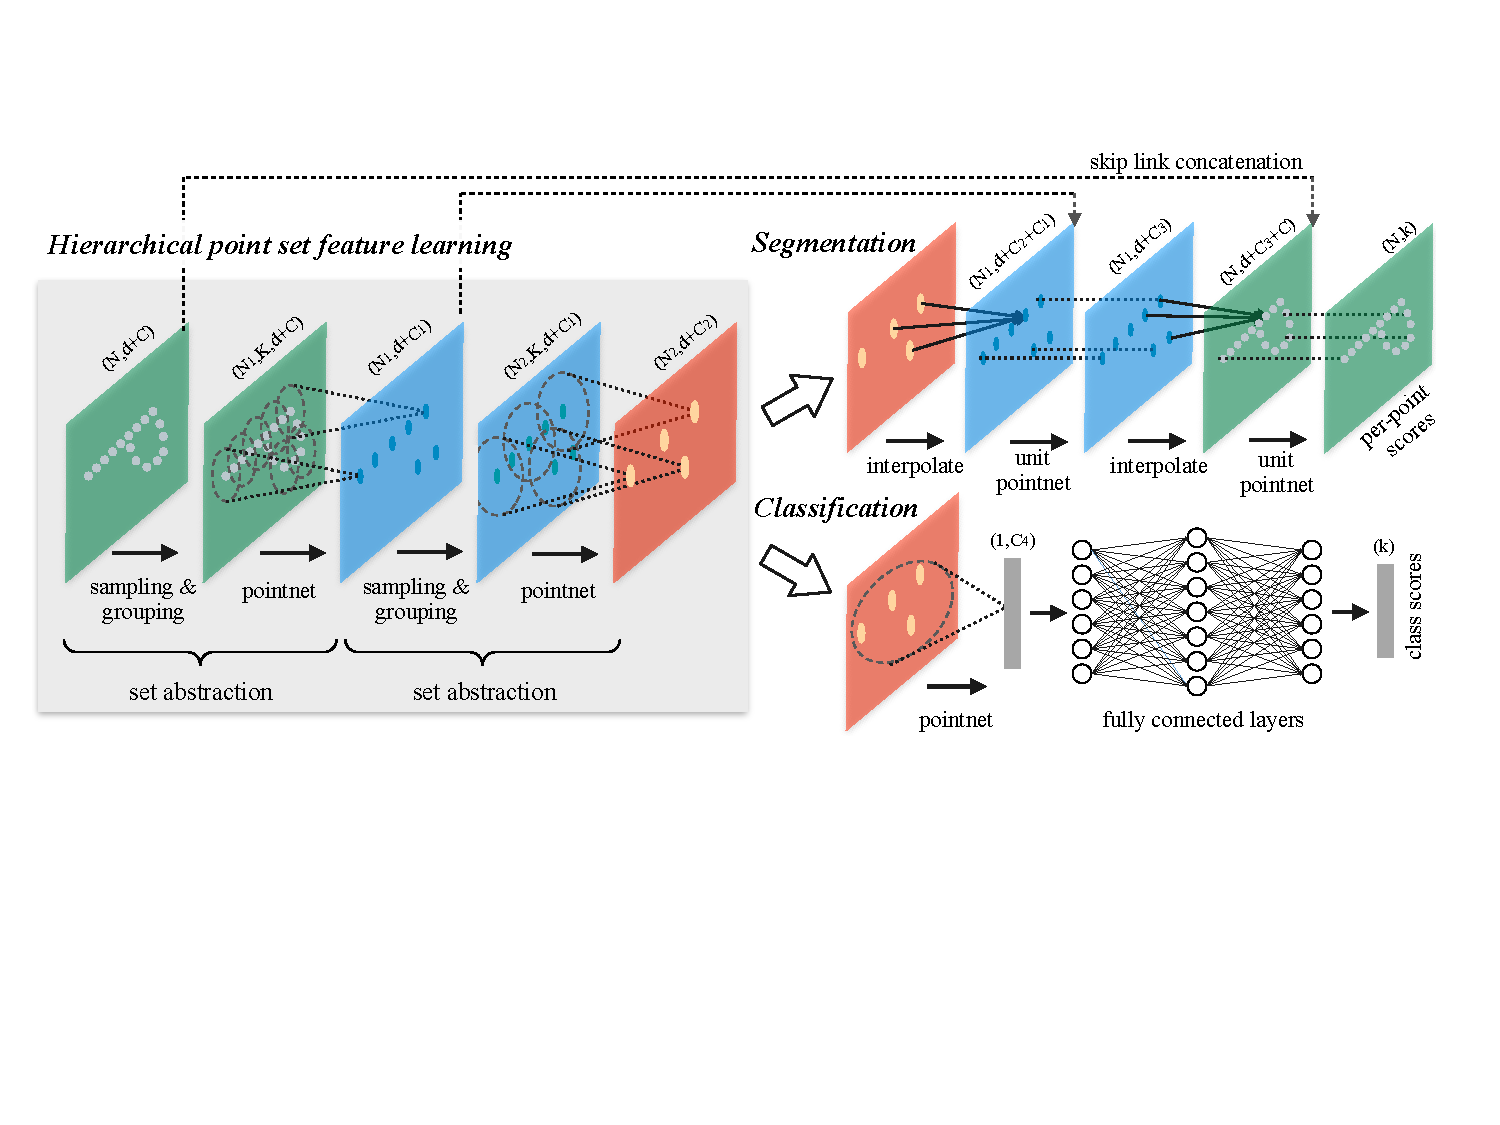
\includegraphics[width=10cm]{./media/_pointnet/pnpp.pdf}
  \caption{Hierarchical feature learning architecture in PointNet++.}
  \label{fig:arch}
\end{figure}
\end{frame}

\begin{frame}
\frametitle{Robust Feature Learning under Non-Uniform Sampling}
\begin{itemize}
  \item PointNet++ uses multi-scale grouping (MSG) and multi-resolution grouping (MRG) to handle varying densities.
  \item Adapts to local density changes, improving robustness and detail capture:
  \begin{itemize}
    \item MSG learn to combine the multi-scale features with random input dropout.
    \item MRG combines features by concatenate lower-level layer with raw data processing in the local region.
  \end{itemize}
\end{itemize}
  \begin{figure}
      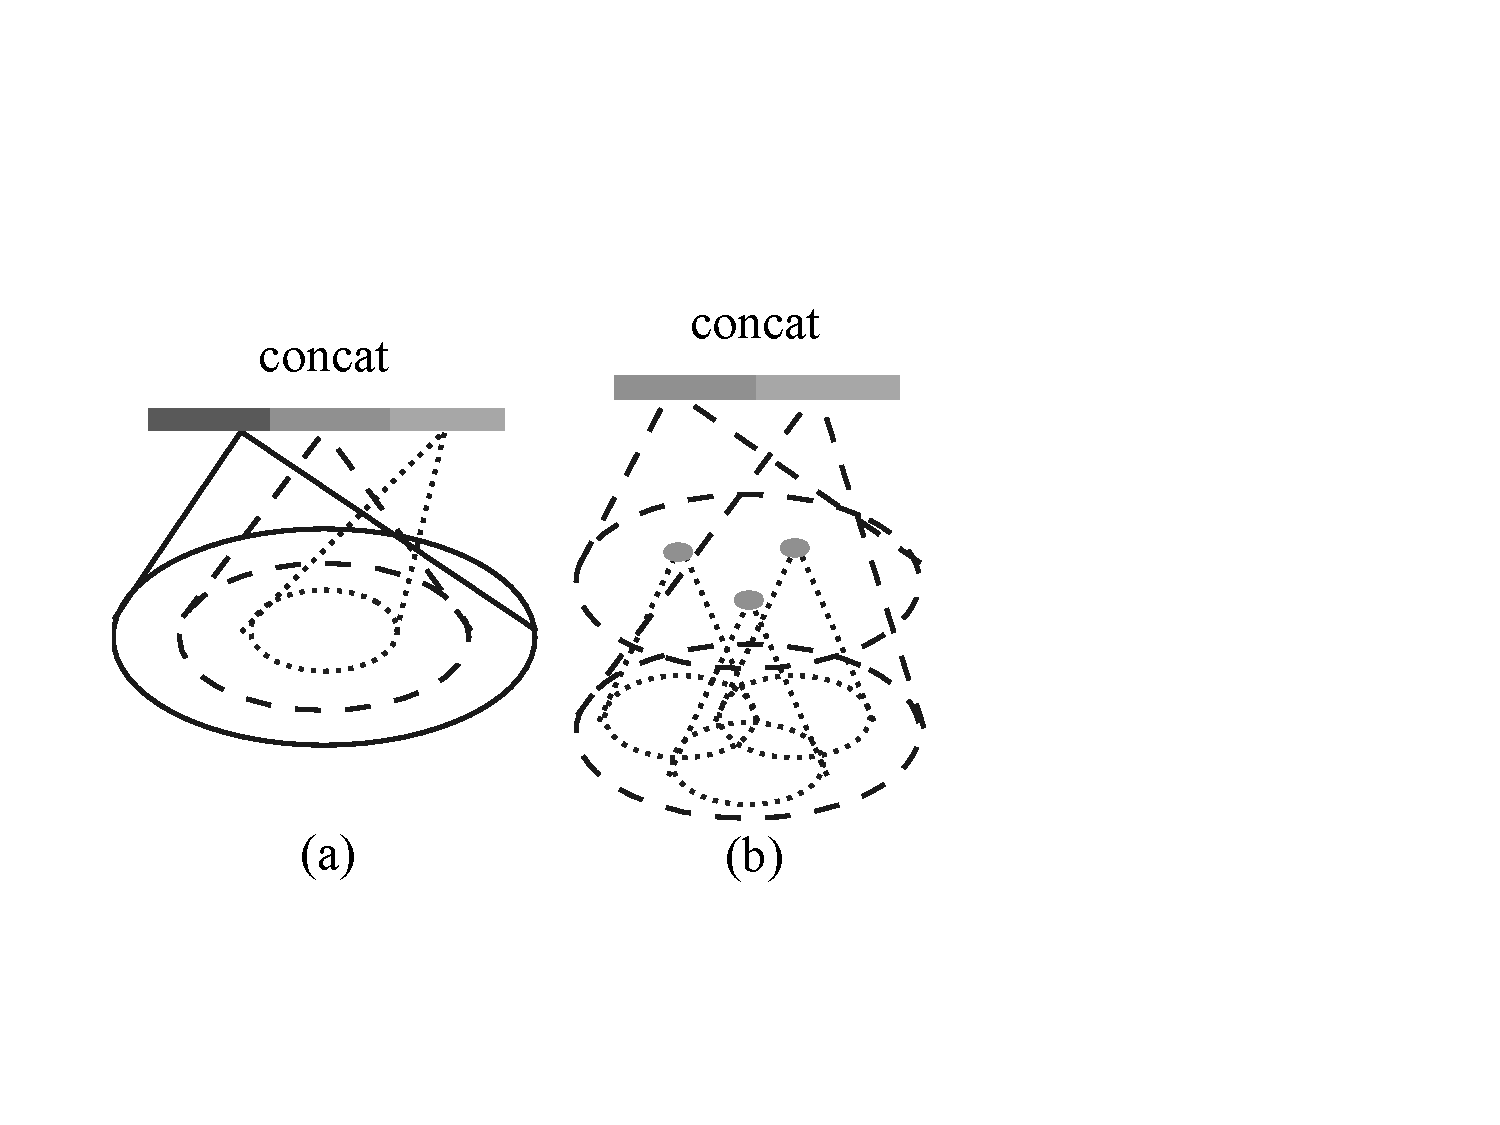
\includegraphics[width=4cm]{./media/_pointnet/multiscale.pdf}
      \caption{Multi-scale and multi-resolution grouping in PointNet++.}
      \label{fig:multiscale}
  \end{figure}
\end{frame}

\begin{frame}
\frametitle{Feature Propagation for Set Segmentation}
\begin{itemize}
  \item Hierarchical feature propagation strategy interpolates features from sampled to original points for original point set for segmentation.
  \item Inverse distance weighting for KNN, MLP with ReLu for feature update. Repeated until get back the original point set with sematic features:
  \begin{equation}
    f^{(j)}(x) = \frac{\sum_{i=1}^{k}w_i (x) f_i^{(j)}}{\sum_{i=1}^k w_i (x)}
    \quad \text{where}\quad w_i(x) = \frac{1}{d(x,x_i)^p},\; j=1,...,C
  \end{equation}
\end{itemize}
\end{frame}

\begin{frame}
\frametitle{Experiments: Overview of Datasets}
\begin{itemize}
    \item \textbf{MNIST:} 60k training and 10k testing samples of handwritten digits.
    \item \textbf{ModelNet40:} 9,843 training and 2,468 testing samples of 3D CAD models.
    \item \textbf{SHREC15:} 1,200 shapes from 50 categories, using five-fold cross-validation.
    \item \textbf{ScanNet:} 1,513 scanned and reconstructed indoor scenes with 1,201 for training and 312 for testing.
\end{itemize}
\end{frame}

\begin{frame}
\frametitle{Classification Experiments on MNIST and ModelNet40}
\begin{itemize}
    \item Evaluated on MNIST (2D) and ModelNet40 (3D).
    \item \textbf{MNIST:} Images converted to 2D point clouds.
    \item \textbf{ModelNet40:} 3D point clouds sampled from mesh surfaces.
    \item Networks trained with 512 points for MNIST and 1024 points for ModelNet40.
    \item Additional features and more points used for higher performance.
    \item Evaluating Robustness to Point Density Variation 
    \begin{itemize}
      \item Test robustness by randomly dropping points during test, reducing point density.
      \item Effectiveness of multi-scale and resolution strategies.
  \end{itemize}
\end{itemize}
\end{frame}

\begin{frame}
\frametitle{Semantic Scene Labeling Experiment on ScanNet Dataset}
\begin{itemize}
    \item Goal: Predict semantic labels for points in indoor scans.
    \item Compared with baselines on the ScanNet dataset.
    \item Hierarchical feature learning captures multi-scale geometric features.
\end{itemize}
% \begin{figure}
%     \centering
%     \includegraphics[width=0.8\linewidth]{example-image-d} % Replace with actual image
%     \caption{Labeling accuracy comparison on real and virtual scans.}
% \end{figure}
\end{frame}

% \begin{frame}
% \frametitle{Visualization of Feature Learning on 3D Point Clouds}
% \begin{itemize}
%     \item Visualization of learned 3D point cloud patterns from ModelNet40.
%     \item Illustrates the network's ability to recognize various geometric features.
% \end{itemize}
% % \begin{figure}
% %     \centering
% %     \includegraphics[width=0.8\linewidth]{example-image-e} % Replace with actual image
% %     \caption{Learned patterns highlighting planes, lines, and corners.}
% % \end{figure}
% \end{frame}

\begin{frame}
\frametitle{Point Set Classification in Non-Euclidean Metric Space}
\begin{itemize}
    \item Metric Space and Intrinsic Features: Using geodesic distances to create a metric space and intrinsic features like WKS, HKS, enabling classification despite pose variations.

    \item Methodology and Implementation: Constructs a geodesic metric space, samples and groups points based on this space, and uses PointNet++ to learn multi-scale intrinsic structures
  
    \item Performance and Results: Outperforms state-of-the-art approaches
\end{itemize}
% \begin{figure}
%     \centering
%     \includegraphics[width=0.8\linewidth]{example-image-d} % Replace with actual image
%     \caption{Labeling accuracy comparison on real and virtual scans.}
% \end{figure}
\end{frame}

\end{document}